
\documentclass[11pt,a4paper]{report}%especifica o tipo de documento que tenciona escrever: carta, artigo, relatório... neste caso é um relatório
% [11pt,a4paper] Define o tamanho principal das letras do documento. caso não especifique uma delas, é assumido 10pt
% a4paper -- Define o tamanho do papel.
\usepackage{graphicx}
\usepackage[portuges]{babel}%Babel -- irá activar automaticamente as regras apropriadas de hifenização para a língua todo o
                                   %-- o texto gerado é automaticamente traduzido para Português.
                                   %  Por exemplo, “chapter” irá passar a “capítulo”, “table of contents” a “conteúdo”.
                                   % portuges -- específica para o Português.
\usepackage[utf8]{inputenc} % define o encoding usado texto fonte (input)--usual "utf8" ou "latin1

\usepackage{graphicx} %permite incluir graficos, tabelas, figuras
\usepackage{url} % para utilizar o comando \url{}
\usepackage{enumerate} %permite escolher, nas listas enumeradas, se os iems sao marcados com letras ou numeros-romanos em vez de numeracao normal

%\usepackage{apalike} % gerar biliografia no estilo 'named' (apalike)

\usepackage{color} % Para escrever em cores
\usepackage{hyperref}

\usepackage{multirow} %tabelas com multilinhas
\usepackage{array} %formatação especial de tabelas em array

\usepackage[pdftex]{hyperref} % transformar as referências internas do seu documento em hiper-ligações.

%Exemplos de fontes -- nao e vulgar mudar o tipo de fonte
%\usepackage{tgbonum} % Fonte de letra: TEX Gyre Bonum
%\usepackage{lmodern} % Fonte de letra: Latin Modern Sans Serif
%\usepackage{helvet}  % Fonte de letra: Helvetica
%\usepackage{charter} % Fonte de letra:Charter

\definecolor{saddlebrown}{rgb}{0.55, 0.27, 0.07} % para definir uma nova cor, neste caso 'saddlebrown'

\usepackage{listings}  % para utilizar blocos de texto verbatim no estilo 'listings'
%paramerização mais vulgar dos blocos LISTING - GENERAL
\lstset{
	basicstyle=\small, %o tamanho das fontes que são usadas para o código
	numbers=left, % onde colocar a numeração da linha
	numberstyle=\tiny, %o tamanho das fontes que são usadas para a numeração da linha
	numbersep=5pt, %distancia entre a numeração da linha e o codigo
	breaklines=true, %define quebra automática de linha
    frame=tB,  % caixa a volta do codigo
	mathescape=true, %habilita o modo matemático
	escapeinside={(*@}{@*)} % se escrever isto  aceita tudo o que esta dentro das marcas e nao altera
}
%
%\lstset{ %
%	language=Java,							% choose the language of the code
%	basicstyle=\ttfamily\footnotesize,		% the size of the fonts that are used for the code
%	keywordstyle=\bfseries,					% set the keyword style
%	%numbers=left,							% where to put the line-numbers
%	numberstyle=\scriptsize,				% the size of the fonts that are used for the line-numbers
%	stepnumber=2,							% the step between two line-numbers. If it's 1 each line
%											% will be numbered
%	numbersep=5pt,							% how far the line-numbers are from the code
%	backgroundcolor=\color{white},			% choose the background color. You must add \usepackage{color}
%	showspaces=false,						% show spaces adding particular underscores
%	showstringspaces=false,					% underline spaces within strings
%	showtabs=false,							% show tabs within strings adding particular underscores
%	frame=none,								% adds a frame around the code
%	%abovecaptionskip=-.8em,
%	%belowcaptionskip=.7em,
%	tabsize=2,								% sets default tabsize to 2 spaces
%	captionpos=b,							% sets the caption-position to bottom
%	breaklines=true,						% sets automatic line breaking
%	breakatwhitespace=false,				% sets if automatic breaks should only happen at whitespace
%	title=\lstname,							% show the filename of files included with \lstinputlisting;
%											% also try caption instead of title
%	escapeinside={\%*}{*)},					% if you want to add a comment within your code
%	morekeywords={*,...}					% if you want to add more keywords to the set
%}

\usepackage{xspace} % deteta se a seguir a palavra tem uma palavra ou um sinal de pontuaçao se tiver uma palavra da espaço, se for um sinal de pontuaçao nao da espaço

\parindent=0pt %espaço a deixar para fazer a  indentação da primeira linha após um parágrafo
\parskip=2pt % espaço entre o parágrafo e o texto anterior

\setlength{\oddsidemargin}{-1cm} %espaço entre o texto e a margem
\setlength{\textwidth}{18cm} %Comprimento do texto na pagina
\setlength{\headsep}{-1cm} %espaço entre o texto e o cabeçalho
\setlength{\textheight}{23cm} %altura do texto na pagina

% comando '\def' usado para definir abreviatura (macros)
% o primeiro argumento é o nome do novo comando e o segundo entre chavetas é o texto original, ou sequência de controle, para que expande
\def\darius{\textsf{Darius}\xspace}
\def\antlr{\texttt{AnTLR}\xspace}
\def\pe{\emph{Publicação Eletrónica}\xspace}
\def\titulo#1{\section{#1}}    %no corpo do documento usa-se na forma '\titulo{MEU TITULO}'
\def\super#1{{\em Supervisor: #1}\\ }
\def\area#1{{\em \'{A}rea: #1}\\[0.2cm]}
\def\resumo{\underline{Resumo}:\\ }

%\input{LPgeneralDefintions} %permite ler de um ficheiro de texto externo mais definições

\title{Introdução ao Processamento de Linguagens Naturais (4º ano de Curso)\\
       \textbf{Trabalho Prático 2}\\ Relatório de Desenvolvimento
       } %Titulo do documento
%\title{Um Exemplo de Artigo em \LaTeX}
\author{José André Martins Pereira\\ (a82880@alunos.uminho.pt) \and Ricardo André Gomes Petronilho\\ (a81744@alunos.uminho.pt)
       } %autores do documento
\date{\today} %data

\begin{document} % corpo do documento
\maketitle % apresentar titulo, autor e data

\begin{abstract}  % resumo do documento
Na unidade curricular de Introdução ao Processamento de Linguagens Naturais do Mestrado integrado em Engenharia Informática foi-nos proposta a análise e uitlização de uma ferramenta intitulada \textbf{\href{https://lxml.de/index.html}{lxml}} e utilizar a mesma no contexto de \textbf{NLP}.
\end{abstract}

\tableofcontents % Insere a tabela de indice
%\listoffigures % Insere a tabela de indice figuras
%\listoftables % Insere a tabela de indice tabelas

\chapter{Introdução} \label{chap:intro} %referência cruzada
Na unidade curricular de Introdução ao Processamento de Linguagens Naturais, do Mestrado integrado de Engenharia Informática, foi-nos proposta a análise da ferramenta \textbf{\href{https://lxml.de/index.html}{lxml}}.\newline A ferramenta lxml XML toolkit trata-se de uma associação Python às bibliotecas da linguagem C, denominadas \textbf{libxml2} e  \textbf{libxslt}. As grandes características desta ferramenta são a velocidade e a integridade dos recursos XML dessas bibliotecas com a simplicidade de uma API Python. \newline Assim, este projeto, tem como principais objetivos, o estudo e análise desta ferramenta, bem como a aplicação da mesma para resolver problemas no contexto  NLP.\newline Deste modo, a ideia do grupo para aplicar a ferramenta \textbf{lxml}, foi desenvolver uma aplicação intitulada de \textbf{xmlstats}, capaz de executar expressões regulares sobre ficheiros \textbf{XML} de websites como \textbf{\href{https://pt.stackoverflow.com}{stackOverflow}}, entre outros. A aplicação destas expressões regulares permite a execução de \emph{queries} interessantes como:
\begin{itemize}
    \item o top \textbf{N} utilizadores com mais \textbf{reputação};
    \item procurar por palavras, frases, em \textbf{posts}, \textbf{comments};
    \item verificar os links ou Ips mais usados nos posts ou comentários
    \item ordenar o nome dos utilizadores alfabeticamente
    \item ...
\end{itemize}{}
Como o utilizador do programa é que decide a expressão regular a aplicar, então existe um infinidade de \emph{queries} possíveis a aplicar aos ficheiros \textbf{XML} de um website ou aplicação. \newline O programa também gera ficheiros \textbf{XML} com o output das \emph{queries} para que estes possam ser utilizador por outras aplicações.


\chapter{Estrutura da ferramenta lxml}
A ferramenta \textbf{lxml} é composta por uma API ElementTree, bastante elegante, com todas as funcionalidades necessárias para ler, processar, e escrever ficheiros \textbf{XML}.\newline A ferramenta internamente divide-se em várias diretorias:
\begin{itemize}
    \item .github: ficheiros de configuração do git
    \item becnhmark
    \item doc
    \item samples
    \item src
    \item tools
\end{itemize}{}

Das diretorias acima, a \textbf{doc} é responsável pela documentação do código, \textbf{samples} ficheiros de teste, \textbf{src} ficheiros do código fonte, tools, ferramentas utilizadas, etc.\newline No entanto, a diretoria mais importante será a \textbf{src}, onde internamente ainda é constituída por diretorias de bibliotecas, ficheiros de configuração de package entre outros.

\chapter{Conceção da Solução}

\section{Objetivo do Programa}
Tal como já foi referenciado anteriormente, o programa trata-se de um executor de expressões regulares sobre ficheiros \textbf{XML}, mais propriamente de websites do \textbf{\href{https://archive.org/download/stackexchange}{StackExchange}}, calculando as ocorrências das mesmas. Os ficheiros \textbf{XML} destes websites são normalmente por:

\begin{itemize}
    \item \textbf{Badges.xml}
    \item \textbf{Comments.xml}
    \item \textbf{Posts.xml}
    \item \textbf{Tags.xml}
    \item \textbf{Users.xml}
    \item \textbf{...}
\end{itemize}{}

\section{Funcionalidades}
Como já foi dito, a funcionalidade central da aplicação \textbf{xmlstats} é execução de uma expressão regular a vários dados \textbf{XML}. No entanto existem duas formas distintas de aplicar a mesma. \newline \newline Uma das formas consiste na aplicação da expressão regular a cada entidade (p.e. \textbf{posts}) e calcular as ocorrências dessa expressão por entidade (p.e no post com Id = "91782" a expressão regular ocorreu 128 vezes). \newline Por exemplo: aplicando a expressão regular da figura \ref{img:regIp}, \textbf{regIP}, que captura endereços IP e procurando por um top 3 de ocorrências da mesma em \textbf{posts - Posts.xml}, a aplicação retorna os três \textbf{posts} onde foram publicados mais endereços IP's, sendo o output o verificado na tabela \ref{tab:outputPorEntidade} mais abaixo.

\begin{table}[h!] %Inserir tabela
\begin{center} %colocar a tabela ao centro
\begin{tabular}{ | c | c | } %desenha a tabela % {formato das colunas} -- 'l' a coluna e alinhada a esquerda;
                                                                              %'r' a coluna e alinhada a direita;
                                                                              %'c' a coluna e centralizada
  \hline  %desenhar uma linha horizontal de comprimento igual ao da tabela
  Id do Post &  Número de ocorrências \\
  \hline
  Id="91782"  & 128 \\
  Id="164489" & 80 \\
  Id="76535" & 60 \\
  \hline
\end{tabular}
\end{center}
\caption{Ocorrências por entidade (neste caso por \textbf{Post})} \label{tab:outputPorEntidade}
\end{table}

\begin{figure}[]
	\centering
	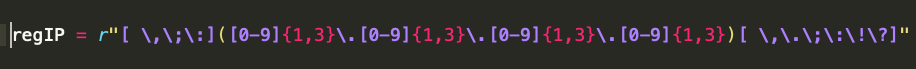
\includegraphics[scale=0.5]{regexIp.png}
	\caption{Expressão regular que captura endereços IP.}
	\label{img:regIp}
\end{figure}

\newpage

A segunda funcionalidade, consiste na aplicação da expressão regular às entidades, no entanto, as ocorrências são guardadas em relação à expressão regular e não à entidade como na funcionalidade anterior. Isto é, o número de vezes que ocorre cada expressão regular em todos os ficheiros. Servindo como exemplo, aplicando a mesma expressão regular apresentada acima, o output desta funcionalidade será o top 3 dos IPs que mais ocorrem nos ficheiros analisados, tal como podemos observar na tabela \ref{tab:outputPorRegex}. 

\begin{table}[h!] %Inserir tabela
\begin{center} %colocar a tabela ao centro
\begin{tabular}{ | c | c | } %desenha a tabela % {formato das colunas} -- 'l' a coluna e alinhada a esquerda;
                                                                              %'r' a coluna e alinhada a direita;
                                                                              %'c' a coluna e centralizada
  \hline  %desenhar uma linha horizontal de comprimento igual ao da tabela
  Expressão regular &  Número de ocorrências \\
  \hline
  '127.0.0.1'  & 357 \\
  '0.0.0.0' & 152 \\
  '192.168.0.7' & 76 \\
  \hline
\end{tabular}
\end{center}
\caption{Ocorrências por expressão regular.} \label{tab:outputPorRegex}
\end{table}

Por fim, e não menos importante, existe uma terceira funcionalidade que é na verdade uma extensão à funcionalidade que guarda as ocorrências por entidade. A única diferença em relação a esta é que não guarda as ocorrências da regex, mas sim o valor do \textbf{atributo} analisado. \newline Por exemplo, a procura pelo top N posts com maior score, apenas se consegue com esta funcionalidade, pois o valor do atributo, neste caso o \textbf{Score}, que é uma \textbf{TAG} do ficheiro \textbf{Posts.xml} é guardado e não as ocorrências da expressão regular utilizada, a tabela \ref{tab:top3MaisScore} apresenta um possível output desta funcionalidade.\newline \newline Importante realçar que as funcionalidades referidas anteriormente da aplicação, após a determinação do número de ocorrências ou do maior atributo (no caso da última funcionalidade), o output das mesmas é guardado num ficheiro em formato \textbf{XML} utilizando a ferramenta \textbf{lxml} numa diretoria chamada \textbf{output}.

\begin{table}[h!] %Inserir tabela
\begin{center} %colocar a tabela ao centro
\begin{tabular}{ | c | c | } %desenha a tabela % {formato das colunas} -- 'l' a coluna e alinhada a esquerda;
                                                                              %'r' a coluna e alinhada a direita;
                                                                              %'c' a coluna e centralizada
  \hline  %desenhar uma linha horizontal de comprimento igual ao da tabela
  Id do Post & Score \\
  \hline
  146  & 56 \\
  4017 & 54 \\
  4188' & 48 \\
  \hline
\end{tabular}
\end{center}
\caption{Top 3 de posts com maior score.} \label{tab:top3MaisScore}
\end{table}

\newpage

\section{Implementação}

Para implementar as funcionalidades descritas acima foram necessárias cinco funções denominadas:
\begin{itemize}
    \item from\_xml(filename :str)
    \item to\_xml(lst : list, agregation : str, single : str)
    \item top\_reg\_by\_elem(filenames : list, attributes : list, regex : str, N : int, keyAttr : int)
    \item top\_reg\_in\_file(filenames : list, attributes : list, regex : str, N : int)
    \item top\_reg\_sort\_by\_atribute(filenames : list, attributes : list, regex : str, N : int, keyAttr : int, castInt: bool)
\end{itemize}{}

A função \textbf{from\_xml} tem como objetivo ler um ficheiro \textbf{XML} e preencher a estrutura \textbf{ElementTree} da ferramenta \textbf{lxml} com o seu conteúdo no formato da mesma.
\newline \newline
A função \textbf{to\_xml} tem o comportamento oposto à anterior, ou seja, escreve no ficheiro, com o formato \textbf{XML} utilizando a ferramenta \textbf{lxml}.\newline
\newline A função \textbf{top\_reg\_by\_elem} tem como objetivo aplicar uma expressão regular a uma \textbf{list} de ficheiros \textbf{XML}, ou seja, o argumento \textbf{filename}, onde respetivamente a cada ficheiro se atibuí um atributo da list \textbf{attributes} que se trata do campo onde se vai buscar o texto (p.e. "Body" no ficheiro Posts.xml, "Text" no ficheiro Comments.xml, etc.). A este texto, presente em cada entidade (p.e. tag \textbf{post}) é aplicado a expressão regular dada como argumento \textbf{regex}. O número de ocorrências da mesma, em cada entidade, é guardado num dicionário onde a chave é o Id da entidade, e o valor, o respetivo número de ocorrências da \textbf{regex}.\newline
\newline Em relação à função \textbf{top\_reg\_in\_file} de forma semelhante, aplica a expressão regular \textbf{regex} a cada entidade, no entanto a grande diferença em relação à funcionalidade anterior é no momento de guardar no dicionário, o número de ocorrências (valor ou value), é associado à expressão regular (chave ou key) e não à entidade (p.e. \textbf{post}). O código desta função é apresentado e explicado na figura \ref{img:top_reg_by_elem}. \newline \newline Por fim, e não menos importante, a função \textbf{top\_reg\_sort\_by\_atribute} é uma extensão da função \textbf{top\_reg\_by\_elem}, sendo que a principal diferença é no momento de guardar os valores no dicionário, onde na função \textbf{top\_reg\_by\_elem}, guarda-se as ocorrências da \textbf{regex} por entidade, enquanto que na \textbf{top\_reg\_sort\_by\_atribute}, tal como o nome sugere, guarda-se o valor do atributo da entidade. Desta forma, esta funcionalidade permite fazer ordenações pelo valor do atributo, como por exemplo o top N de posts com maior score.

\begin{figure}[]
	\centering
	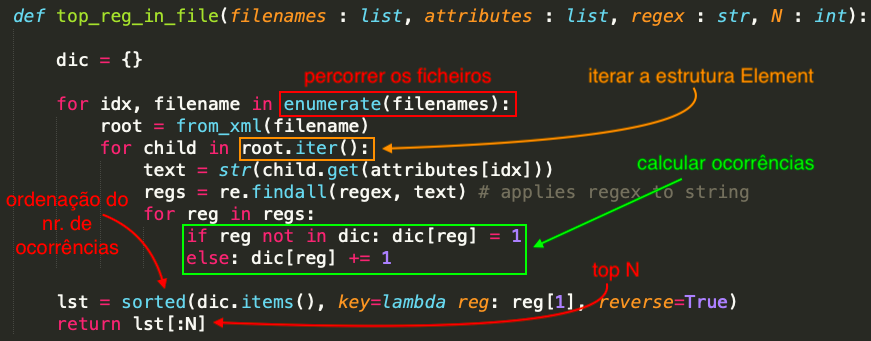
\includegraphics[scale=0.6]{f1.png}
	\caption{Função \textbf{top\_reg\_by\_elem} .}
	\label{img:top_reg_by_elem}
\end{figure}
\chapter{Como instalar e executar o xmlstats}
\section{Requisitos}
\begin{itemize}
    \item Python 3
    \item lxml (ver figura \ref{img:lxml})
    \item Package de scripts do xmlstats (enviados juntamente com este relatório)
    \item Ficheiros .xml (descarregar em \href{https://archive.org/download/stackexchange}{stackexchange})
\end{itemize}{}

\begin{figure}[h]
	\centering
	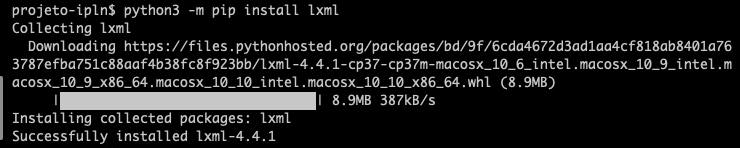
\includegraphics[scale=0.6]{lxml.png}
	\caption{Instalação do lxml .}
	\label{img:lxml}
\end{figure}

\section{Como executar}
Para execução do programa e caso a equipa não tenha colocado a pasta \textbf{data} no (.zip) com os ficheiros de teste (.xml), deverá descarregar os mesmos, no entanto recomendamos ir ao seguinte website \textbf{\href{https://archive.org/download/stackexchange}{StackExchange}} e procurar por \textbf{StackOverflow}. Para facilitar o processo de execução, a equipa desenvolveu um \textbf{makefile} que se pode ver nas figuras \ref{img:mk1}, \ref{img:mk2}, \ref{img:mk3} e \ref{img:mk4}, onde se pode substituir os argumentos necessários para execução do programa. O makefile ainda é composto para auxílio de algumas macros de execução para se entender como se executa o \textbf{xmlstats}. Os argumentos necessários são:
\begin{itemize}
    \item -t (0 para executar funcionalidade por entidade, 1 para a funcionalide por expressão regular, 2 para executar a expressão regular e ordenar pelo valor do atributo)
    \item -f (pode ser um único ficheiro ou uma lista, do tipo 'file1, file2, fil3')
    \item -a  (atributos das tags de cada ficheiro respetivamente 'atr1,atr2,atr3')
    \item -r expressão regular
    \item -c (apenas na opção -t = 2 necessita desteargumento -c, que indica se o atributo da tag a analisar é inteiro (-c 1), caso contrário (-c 0)
    \item -l limite para top N
\end{itemize}{}
\begin{figure}[h]
	\centering
	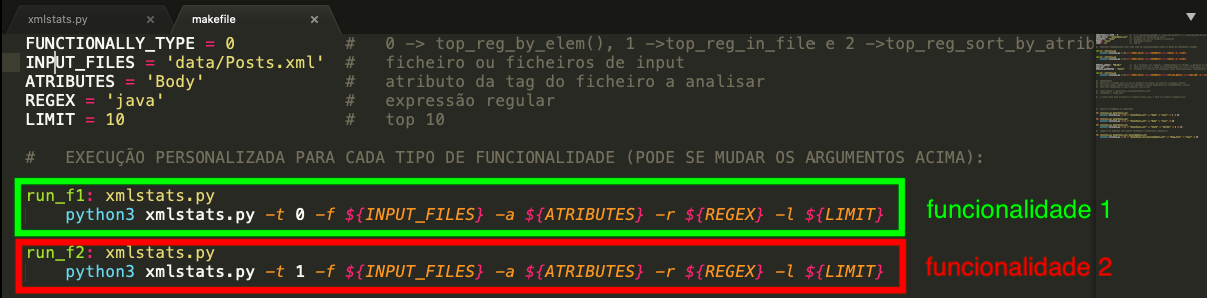
\includegraphics[scale=0.40]{mk1.png}
	\caption{Ficheiro makefile, funcionalidade 1 e 2.}
	\label{img:mk1}
\end{figure}

\begin{figure}[h]
	\centering
	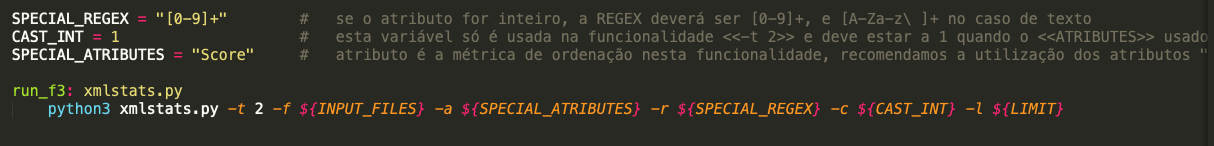
\includegraphics[scale=0.40]{mk2.png}
	\caption{Ficheiro makefile, funcionalidade 3.}
	\label{img:mk2}
\end{figure}

\begin{figure}[h]
	\centering
	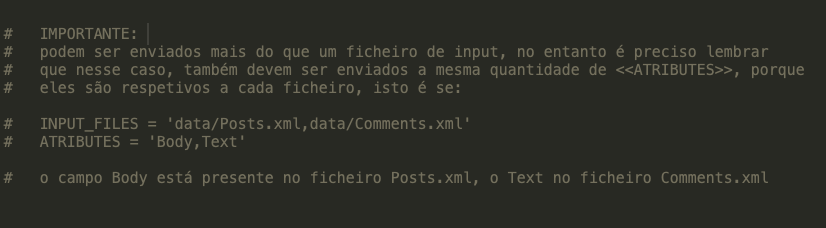
\includegraphics[scale=0.40]{mk3.png}
	\caption{Ficheiro makefile, notas importantes.}
	\label{img:mk3}
\end{figure}

\begin{figure}[h]
	\centering
	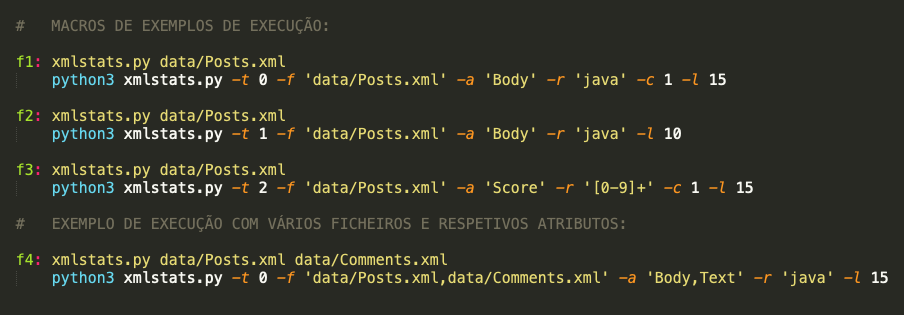
\includegraphics[scale=0.40]{mk4.png}
	\caption{Ficheiro makefile, macros de execução.}
	\label{img:mk4}
\end{figure}

A figura \ref{img:1}, apresenta-se a execução deste programa ao ficheiro Posts.xml, onde o atributo analisado é o Body, presente nas tags deste ficheiro, a expressão regular é a palavra \textbf{java}, e o output é apresentado em formato tabelar, produzido por uma função denominada \textbf{pretty\_print}, onde, neste exemplo, o valor da esquerda representa o id do Post e o da direita o número de ocorrências da expressão regular.\newline \newline De seguida, apresentam-se as restantes funcionalidades em execução e a respetiva explicação na legenda das imagens (figuras \ref{img:1}, \ref{img:2} e \ref{img:3}).

\begin{figure}[h]
	\centering
	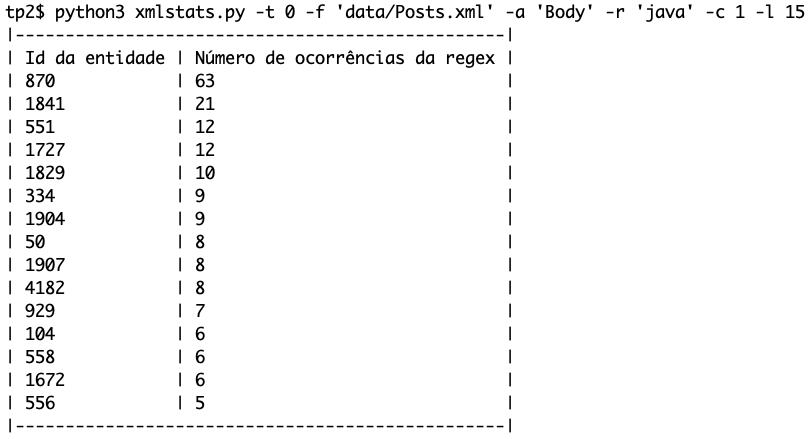
\includegraphics[scale=0.6]{1.png}
	\caption{Executar a expressão regular "java" ao texto do atributo \textbf{Body}, presente na tag post do ficheiro Posts.xml, com a funcionalide -t 0, ou seja, calcula e ordena as ocorrências por entidade. A tabela é escrita em formato XML na diretoria output.}
	\label{img:1}
\end{figure}

\begin{figure}[h]
	\centering
	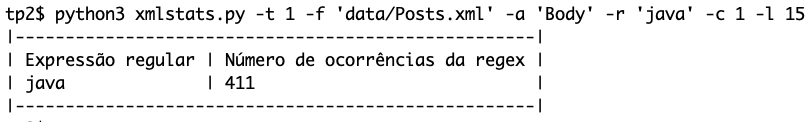
\includegraphics[scale=0.6]{2.png}
	\caption{Executar a expressão regular "java" ao texto do atributo \textbf{Body}, presente na tag post do ficheiro Posts.xml, com a funcionalide -t 1, ou seja, calcula e ordena as ocorrências por expressão regular.A tabela é escrita em formato XML na diretoria output.}
	\label{img:2}
\end{figure}

\begin{figure}[h]
	\centering
	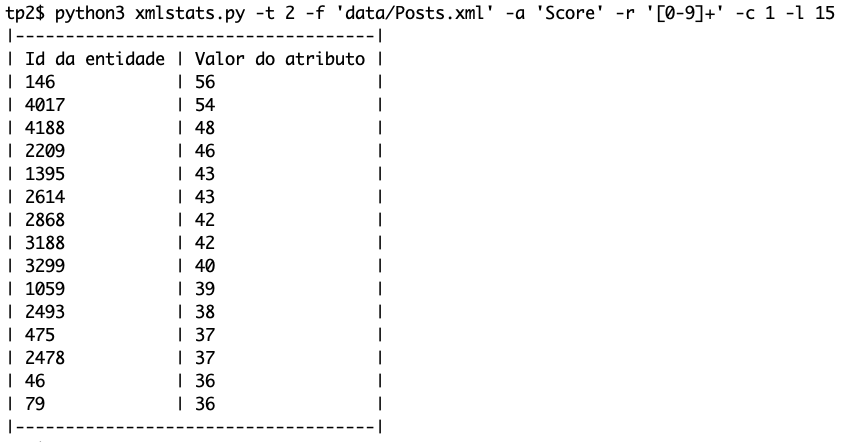
\includegraphics[scale=0.6]{3.png}
	\caption{Executar a expressão regular "[0-9]+" ao texto presente no atributo \textbf{Score}, presente na tag post do ficheiro Posts.xml, com a funcionalide -t 2, ou seja, calcula e ordena pelo atributo \textbf{Score}.A tabela é escrita em formato XML na diretoria output.}
	\label{img:3}
\end{figure}

\chapter{Conclusão} 
Em suma, os objetivos inicialmente propostos foram cumpridos, no entanto a equipa entende que deveria ter estudado melhor a estrutura/componentes internos da ferramenta \textbf{lxml}. \newline No entanto, com uma análise da documentação presente no website da ferramenta, conseguiu-se perceber a excelente \textbf{ElementTree API}, utilizada neste programa, e as diversas funcionalidades que a mesma permite. Percebeu-se também a importância de estudar ferramentas desconhecidas, para reutilização de funcionalidades já existentes e bem testadas.
\newline Por fim, a aplicação inicialmente proposta, \textbf{xmlstats}, que aplica expressões regulares a ficheiros \textbf{XML} foi concretizada com sucesso, permitindo executar diversas \emph{queries} apartir de expressões regular a toda uma estrutura de um website como o \textbf{StackOverflow}.

\end{document} 